%# -*- coding: utf-8-unix -*-
% !TEX program = xelatex
% !TEX root = ../thesis.tex
% !TEX encoding = UTF-8 Unicode
%%==================================================
%% chapter02.tex for SJTU Master Thesis
%% based on CASthesis
%% modified by wei.jianwen@gmail.com
%% Encoding: UTF-8
%%==================================================

\chapter{Modeling and Analysis}
\label{chap:modeling and analysis methods}
In this chapter, a basic model would be introduced for competition on two-layer network. It would be also explained that how each layer is made up and what kind of function and dynamics it has. After modeling, many simulations would be fulfilled under the various conditions. Several indexes would be provided to analyze the interaction between two-layers. Simulation results would be analyzed with these indexes. 
\begin{figure}[!htb]
	\centering
	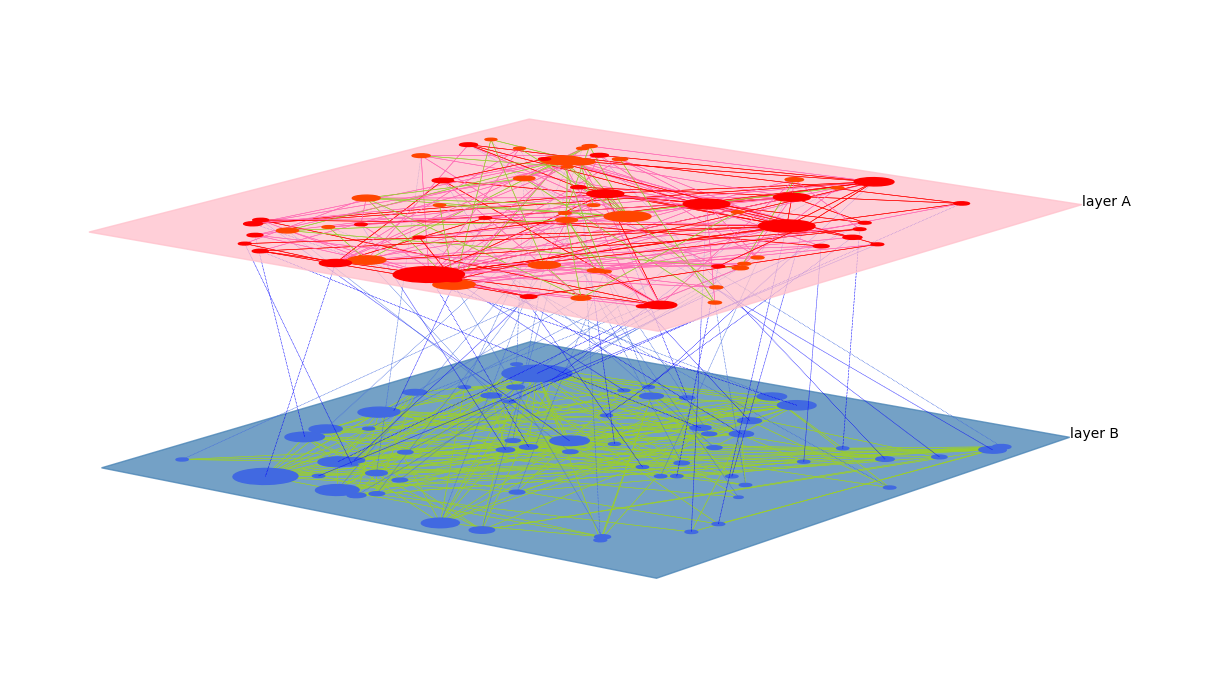
\includegraphics[width=\hsize]{chap2_modeling.png}
	\caption{Competition of Interconnected Network}
	\label{chap2_modeling}
\end{figure}
 
\section{Modeling of two layer network}
\label{sec:modeling of two layer network}
The model consists of two layers, and each layer has different dynamics. For layer A, the node change its states according to $M$ model as introduced in \parencite{rocca2014}. Here, we choose $M=2$, that each node has four states $(-2, -1, +1, +2)$. For each link $(k, j)$ belong to layer A,  the dynamics are designed as follows:
\begin{itemize}
	\item Compromise : if two nodes connected with link$(k, j)$ have opposite orientations, their states become more moderate with probability $q$ :
	\begin{align}
	\mbox{if } S_k<0 \mbox{ and } S_j>0  \Rightarrow (S_k, S_j) \rightarrow (S_k^r, S_j^l) \mbox{ with } prob.q,\\
	\mbox{if } S_k>0 \mbox{ and } S_j<0  \Rightarrow (S_k, S_j) \rightarrow (S_k^l, S_j^r) \mbox{ with } prob.q.
	\end{align}
	If $S_k = \pm1$ and $S_j = \mp1$, one switches orientation at random:
	\begin{align}
	(\pm 1, \mp 1)\rightarrow \left\{\begin{matrix}
	(+1, +1) \mbox{ with } prob.q/2,
	\\(-1, -1)\mbox{ with } prob.q/2.
	\end{matrix}\right.
	\end{align}
		
	\item Persuasion : if two nodes connected with link$(k, j)$ have the same orientation, their states become more extreme with probability $p$ :
	\begin{align}
	\mbox{if } S_k<0 \mbox{ and } S_j<0  \Rightarrow (S_k, S_j) \rightarrow (S_k^l, S_j^l) \mbox{ with } prob.p,\\
	\mbox{if } S_k>0 \mbox{ and } S_j>0  \Rightarrow (S_k, S_j) \rightarrow (S_k^r, S_j^r) \mbox{ with } prob.p.
	\end{align}
\end{itemize}
For each external link $(k,j)$ with $k$ belong to layer A, the state of node $k$ is updated according to :
\begin{itemize}
	\item $S_k \cdot S_j < 0$ :
	\begin{align}
	\mbox{if } S_k<0 \mbox{ and } S_j>0  \Rightarrow (S_k, S_j) \rightarrow (S_k^r, S_j) \mbox{ with } prob.q,\\
	\mbox{if } S_k>0 \mbox{ and } S_j<0  \Rightarrow (S_k, S_j) \rightarrow (S_k^l, S_j) \mbox{ with } prob.q.
	\end{align}
	\item $S_k \cdot S_j > 0$ :
	\begin{align}
	\mbox{if } S_k<0 \mbox{ and } S_j<0  \Rightarrow (S_k, S_j) \rightarrow (S_k^l, S_j) \mbox{ with } prob.p,\\
	\mbox{if } S_k>0 \mbox{ and } S_j>0  \Rightarrow (S_k, S_j) \rightarrow (S_k^r, S_j) \mbox{ with } prob.p.
	\end{align}
\end{itemize}
Here, $S_k^r$ and $S_k^l$ denote the right and left neighboring states of node $k$, defined as
\begin{align}
S_k^r &= \left\{\begin{matrix}
+1,\mbox{ for } S_k = -1\\
+2,\mbox{ for } S_k = +2\\ 
S_k + 1,\mbox{ otherwise }, 
\end{matrix}\right. &
S_k^l &= \left\{\begin{matrix}
-1,\mbox{ for } S_k= +1
\\ -2,\mbox{ for } S_k=-2
\\ S_k - 1,\mbox{ otherwise }.
\end{matrix}\right.
\end{align}

The sign of $S^A$ represents its opinion orientation and its absolute value $|S^A|$ measures the intensity of its opinion. So, $|S^A|=2$ represents a positive or a negative extremist, while  $|S^A|=1$ correspond to a moderate opinion of each side. In case of internal link $(k, j)$ belong to layer A, when the nodes have the same orientation$(S_kS_j>0)$, if the states of nodes are moderate, then they become extreme$(S_k=\pm1 \rightarrow \pm2, S_j= \pm1 \rightarrow \pm2)$ with probability $p$. If they are already extreme, they remain extreme$(S_k=\pm2 \rightarrow \pm2, S_j= \pm2 \rightarrow \pm2)$. On the other hand, when the nodes have opposite orientations$(S_kS_j<0)$, if they are extreme, the states of nodes become moderate$(S_k=\pm2 \rightarrow \pm1, S_j= \pm2 \rightarrow \pm1)$ with probability $q$. If they are already moderate, they switch orientations individually$(S_k=\pm1 \rightarrow \mp1, S_j= \pm1 \rightarrow \mp1)$.  In case of interaction between node in layer A and node in layer B, node in layer A follows opinion dynamics formula, but the state of node in layer B does not change. In other words, the state of layer B affects layer A, but layer A dynamics does not affect the state of node in layer B. For example, one of the layer A node, $S_k = +2$ is connected with  $S_j = -1$ node of layer B. Here, $S_k$ will change into $S_k = +1$ with $prob.q$, but $S_j$ will not change, which indicates that the states of layer B will influence the states of layer A.

The dynamics of layer B follows the decision-making dynamics as introduced in \parencite{abrams2003, vazquez2010}. The state of node i in layer B can be $+1$ and $-1$, and it updates according to

\begin{equation}
{P_B}({S_i} \to  - {S_i}) = \begin{cases}
{\left({\displaystyle\frac{{{i_i} + {e_i}}}{{{n^{ - {S_i}}}}}}\right)}{\cdot}{\left({\displaystyle\frac{{n^{-{S_i}}}}{{{i_i} + {e_i}}}} \right)^{1/v}}  ,\mbox{ if } v \ne 0\\
0,\mbox{ if } v = 0\\
0,\mbox{ if } {n^{ - {S_i}}} = 0
\end{cases},
\end{equation}

where $i_i$ is the number of internal edges and $e_i$ is the number of external edges. $n^{-S_i}$ is the number of neighbors of node $i$ with opposite state $-S_i$. $v$ represents the volatility that measures how prone a node change its state. The scale of $v$ is from $0$ to $1$. If $v \simeq 0$,  a node is unlikely to change its state. On the other hand, if $v \simeq 1$, a node is very likely to change its state. Also, this formula shows that the more the number of edges connected with the nodes of opposite state is, the easier the nodes are to change into the opposite state.\\
\begin{figure}[!htb]
	\centering
	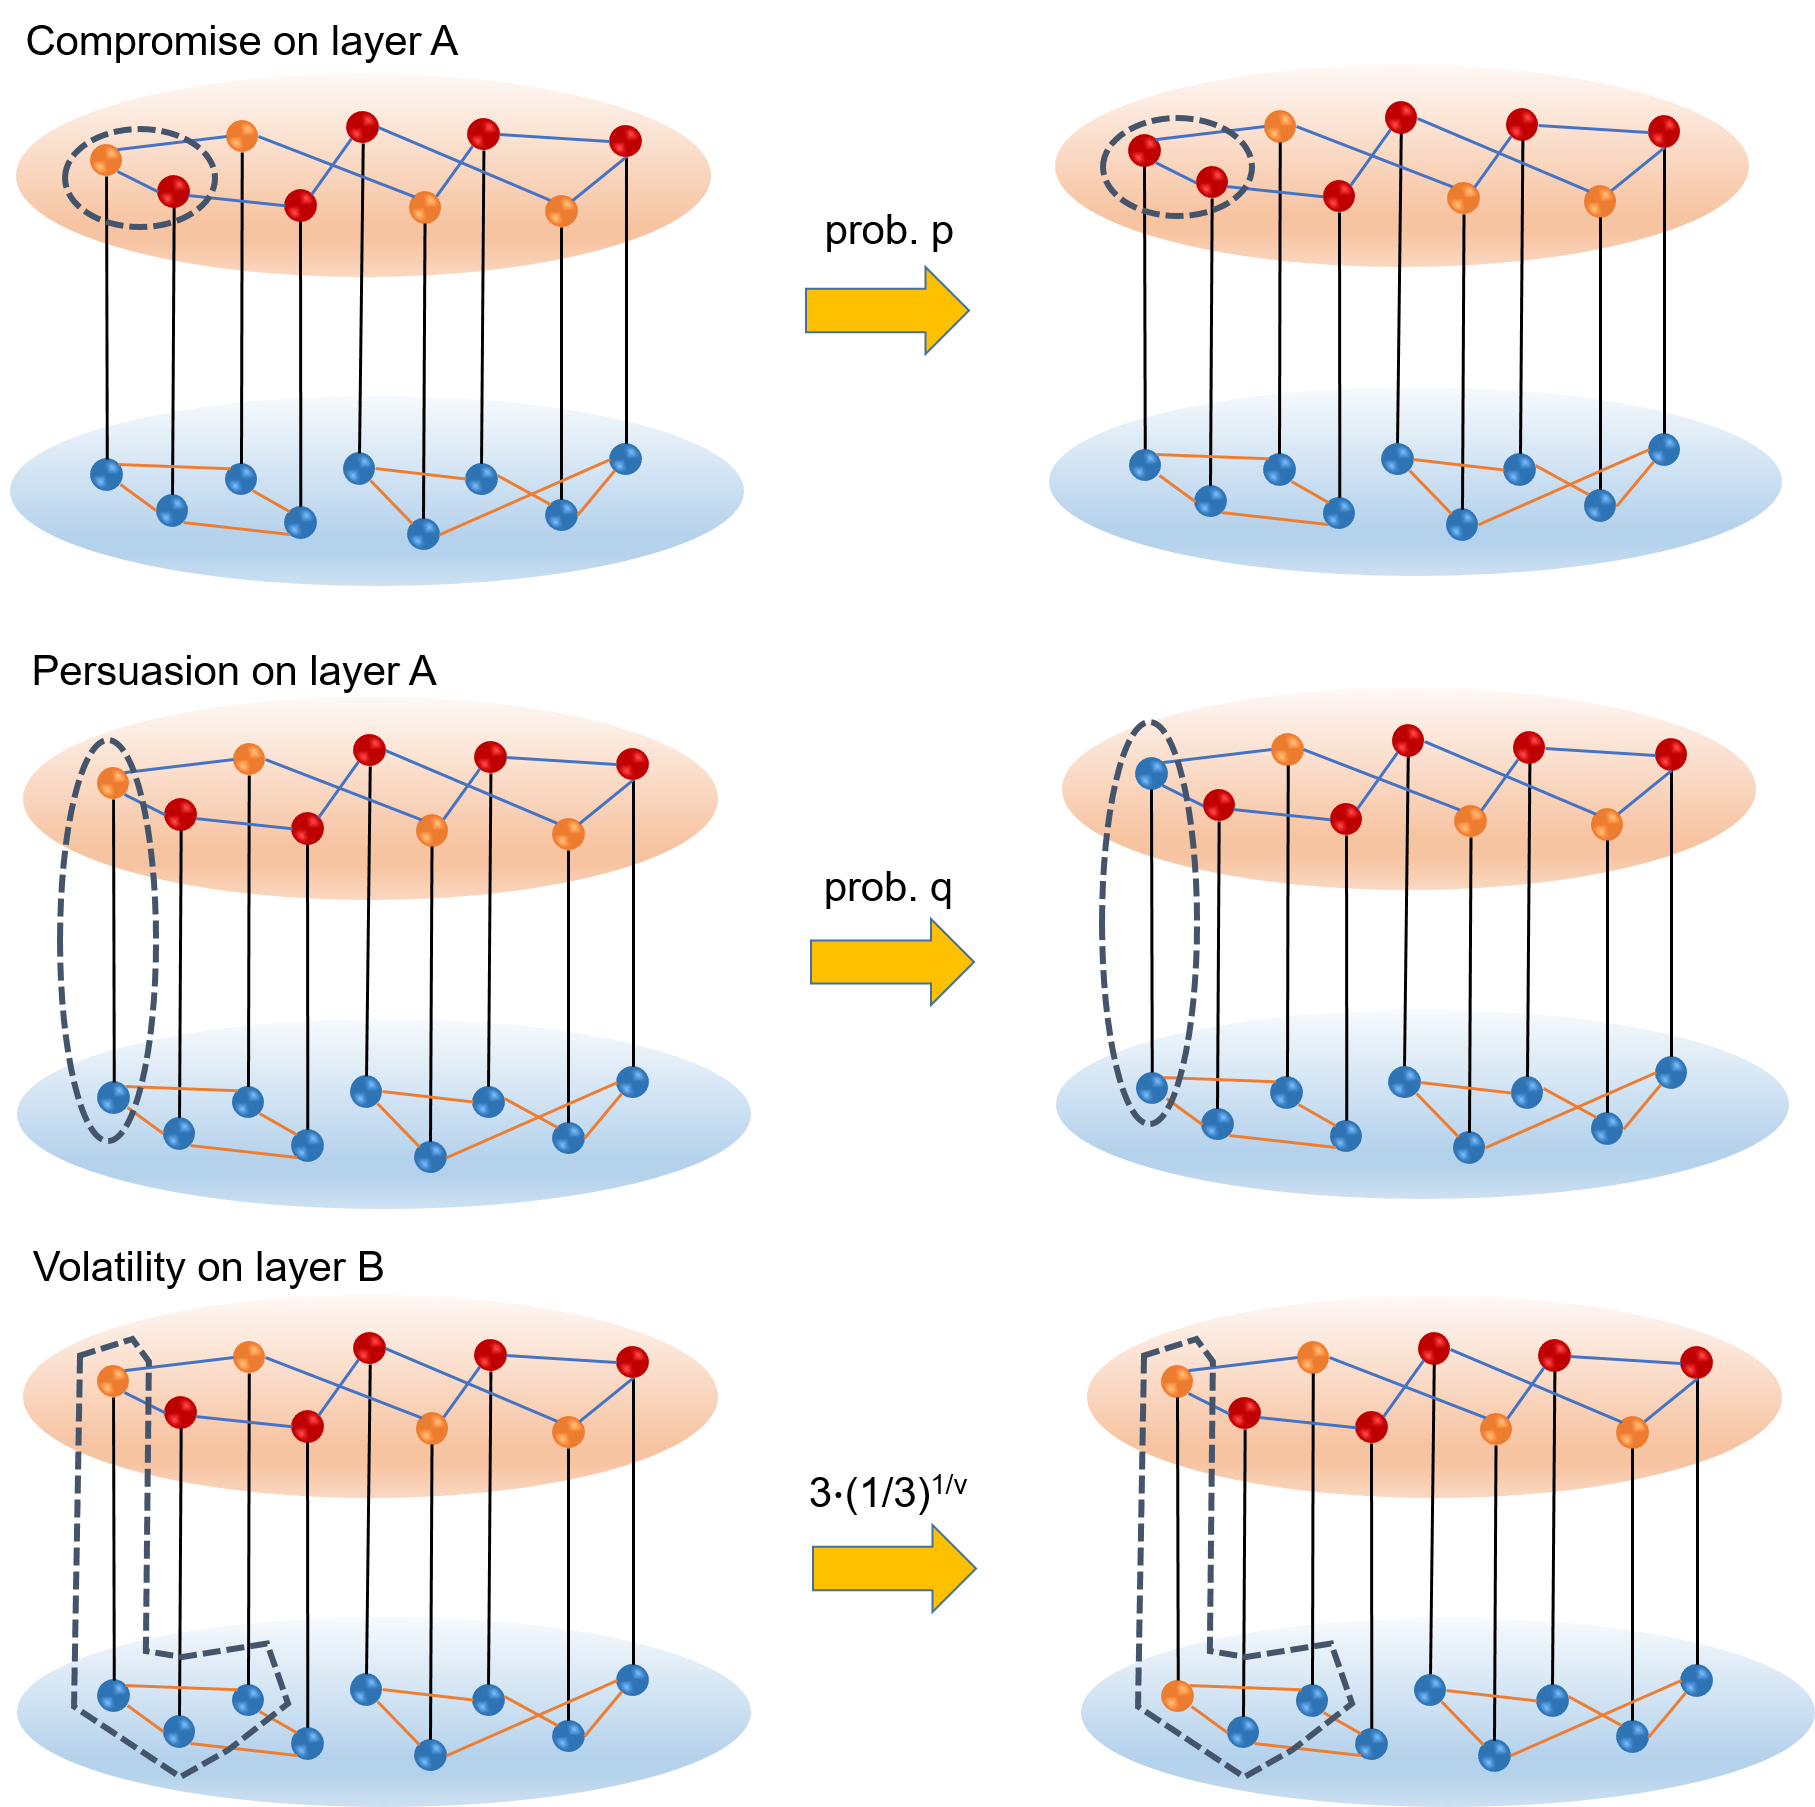
\includegraphics[width=\hsize]{chap2_dynamics.png}
	\caption{Dynamics on two layers}
	\label{chap2_dynamics}
\end{figure}


\section{Simulations and Analysis}
This modeling is nonlinear in that the structure of the model changes with the states of nodes. In this model, helpful mathematical tools are no longer applicable and  it turns out, moreover, that rigorous analytical results are difficult to obtain.\parencite{nicolas2017, rainer2002}. For that reason, we would try to carry out the analysis of the above nonlinear model to a large extent by simulations on the computer.

To start with a polarized competition, as the initial conditions,  nodes in layer A are all positive, and nodes in layer B are all negative as shown in Fig.~\ref{chap2_modeling}. For nodes in layer A, it begins with the status where half of nodes are $+1$ and the others are $+2$. The initial state of nodes in layer B have only $-1$. 

There are two parameters, $p$ and $q$ in the dynamics of layer A. To simply represent the probability $p$ and probability $q$ together, we set $p+q=1$. So, $p$ represents the reinforcement or strength of opinion such as extreme or moderate, which is scaled to be $0$ to $1$. And, there are only 1 parameter, $v$ in the dynamics of layer B. The scale of $v$ is also $0$ to $1$ as $p$. $v$ represents the volatility, which means how prone the state can be changed into the opposite state.  

To implement the interconnected dynamics, one step consists of two layers dynamics, where every node in layer A is checked with opinion dynamics, and every node in layer B updates its state according to the decision-making dynamics. Basically, the dynamics order follows updating state of layer B after updating state of layer A. The dynamics orders and time-related updating rules would be discussed specifically in chapter 4.      

Each simulation takes $100$ steps, and $100$ simulations are considered for average results. To analyze the simulation results, we use \textit{`Average State'(AS)} to measure the average states of network and \textit{`Consensus Index'(CI)} to measure how close the states of network is to consensus. 

\begin{equation}
AS = avg\left( {\sum\limits_i^{{K^A}} {S_i^A/4} } \right) + avg\left( {\sum\limits_i^{{K^B}} {S_i^B/2} } \right).
\end{equation}

\begin{equation}
CI = \frac{{({K_ + }^A \cdot {K_ - }^B) + ({K_ - }^A \cdot {K_ + }^B)}}{{{K^A} \cdot {K^B}}}.
\end{equation}

In these formula, $S_i^A$ means the state of node \textit{i} in layer A, and $K^A$ is the number of nodes in layer A. ${K_ + }^A$ represents the number of nodes with positive state in layer A.   

With \textit{AS}, it could be verified whether the consensus happens in accordance with the change of $p$ and $v$.  If the positive consensus happens, it would be close to the value of $+1$ and if the negative consensus happens, it would be close to the value of $-1$. And, the medium values between $+1$ and $-1$ mean the states are belonging to the coexistence or dissent part.
\begin{figure}[!htb]
	\centering
	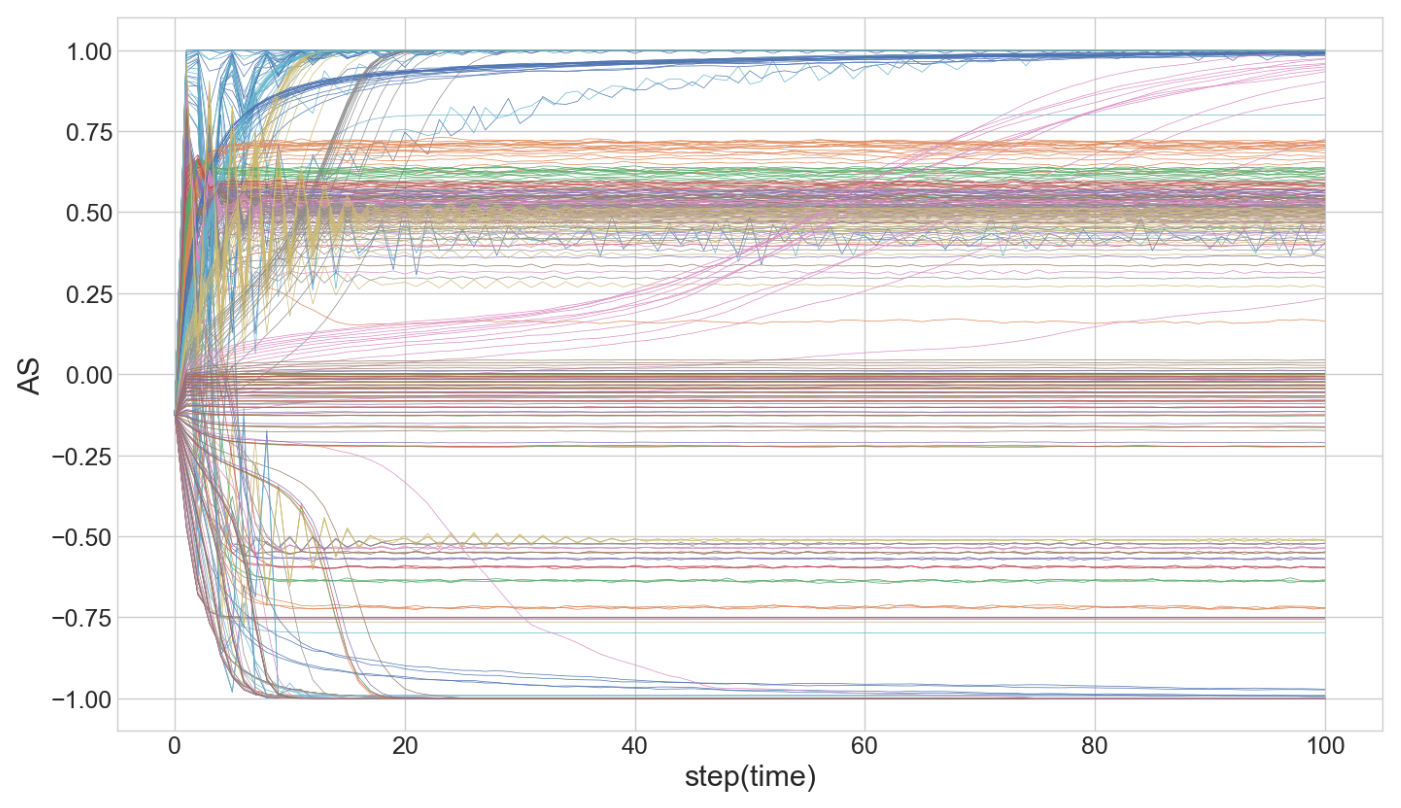
\includegraphics[width=\hsize]{chap2_timeflow_AS(BA3_BA3).png}
	\caption{AS values per each step according to all parameters}
	\label{chap2_timeflow_AS(BA3_BA3)}
\end{figure}
Fig.~\ref{chap2_timeflow_AS(BA3_BA3)} shows that AS values are convergent to $+1$, $-1$ or other values as step(time) goes by. $+1$ means making positive consensus. $-1$ means making negative consensus. The other values mean coexistence or dissent state. 

With \textit{CI}, it could be measured how close the network state is to consensus. If the \textit{CI} is close to $0$, the state is close to positive or negative consensus. If the \textit{CI} is close to $1$, the state is the separated coexistence where states of all nodes in layer A is opposed to states of all nodes in layer B. If the CI is close to $0.5$, the state is the mixed coexistence where each layer has both positive and negative states of nodes.

\begin{figure}[!htb]
	\centering
	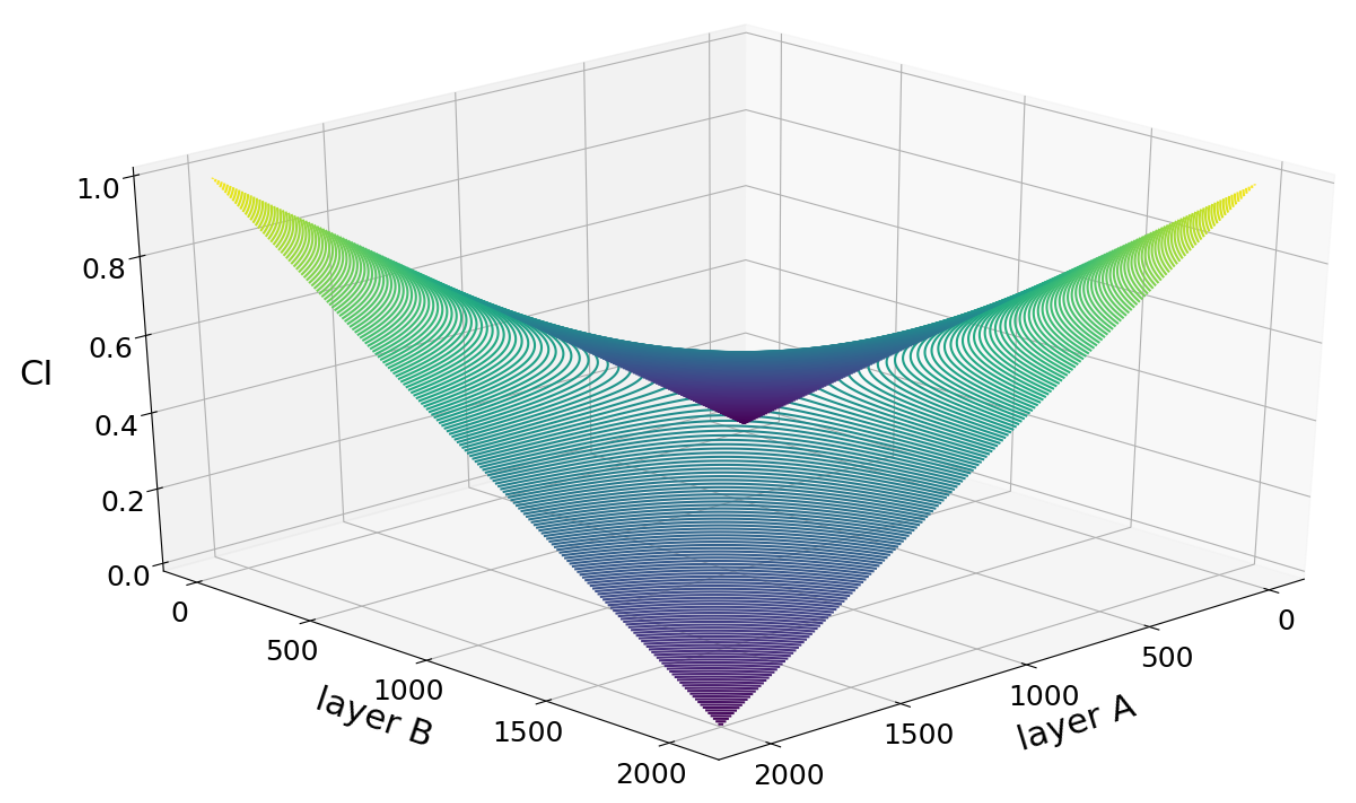
\includegraphics[width=\hsize]{chap2_CI_values.png}
	\caption{CI values according to all ${K_ + }^A$ and ${K_ + }^B$  }
	\label{chap2_CI_values}
\end{figure}
Fig.~\ref{chap2_CI_values} shows the characteristics of \textit{CI}. Same orientation states in two layers make \textit{CI} $0$. Opposite orientation states between two layers make \textit{CI} $1$. And mixed states in two layers make \textit{CI} close to $0.5$. 

\begin{figure}[!htb]
	\centering
	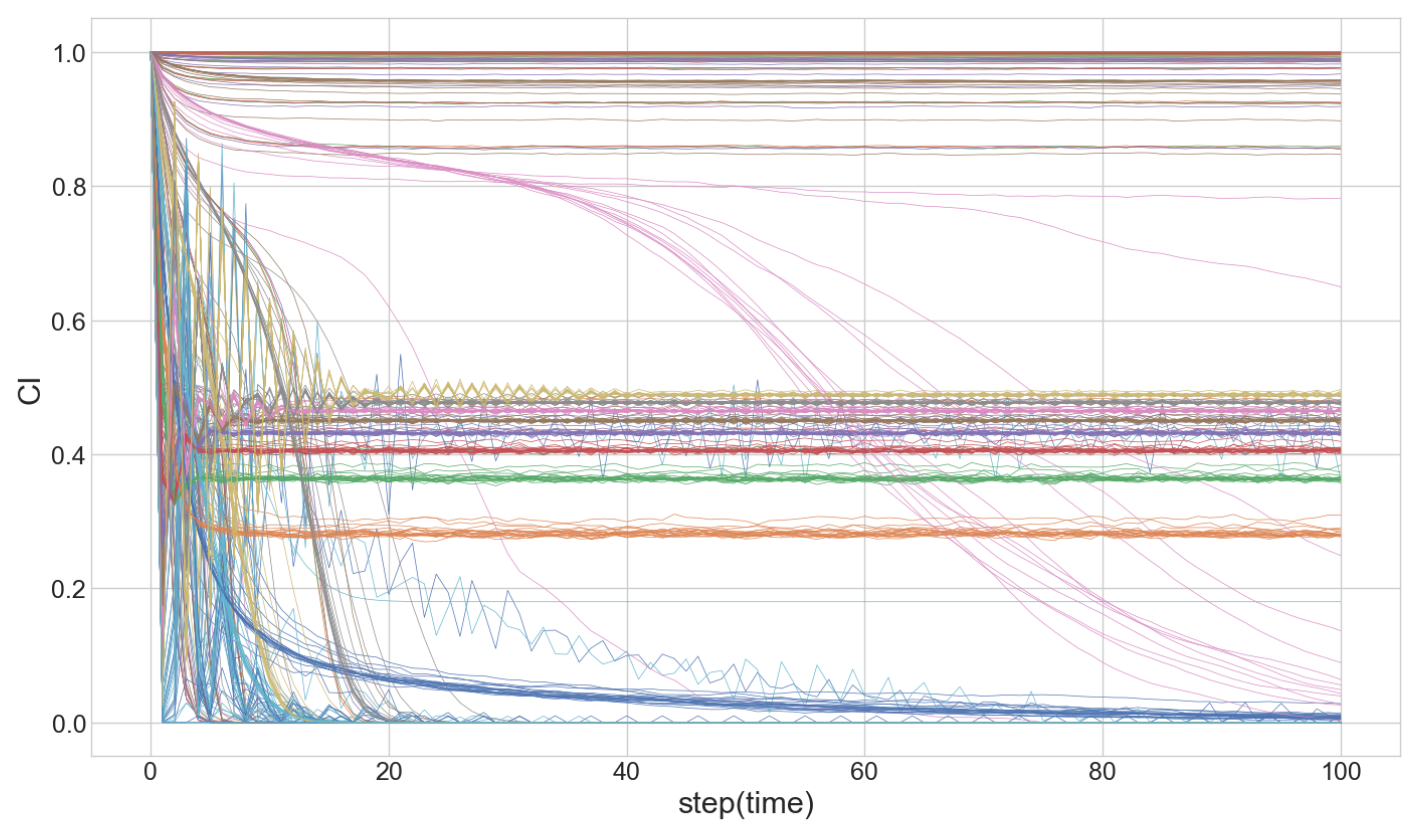
\includegraphics[width=\hsize]{chap2_timeflow_CI(BA3_BA3).png}
	\caption{CI values according to all ${K_ + }^A$ and ${K_ + }^B$  }
	\label{chap2_timeflow_CI(BA3_BA3)}
\end{figure}
As Fig.~\ref{chap2_timeflow_CI(BA3_BA3)} shown, \textit{CI} values are convergent to $+1$, $0$, or other values as step(time) goes by. $0$ means positive or negative consensus. $+1$ means opposite state between two layers. The other values means mixed state. By using \textit{CI}, coexistence states can be divided into two categories, separated state and mixed state.   

To measure and evaluate the consensus results regarding to two parameters $p$ and $v$, we use four kinds of indexes including \textit{`AS total'}, \textit{`Positive Consensus Ratio'(PCR)}, \textit{`Negative Consensus ratio'(NCR)}, and \textit{`Consensus Ratio'(CR)}. \textit{AS total} means the summation of \textit{AS} for all $p$s and all $v$s. \textit{PCR} is the ratio of positive consensus over all simulations. Similarly, \textit{NCR} is the ratio of experiments with negative consensus. \textit{CR} is the ratio of experiments reaching consensus, i.e. summation of \textit{PCR} and \textit{NCR}.

\begin{equation}
\begin{array}{cl}
AS\mbox{ \textit{total} } = \frac{{\sum\limits_j^m {\sum\limits_i^n {A{S_{{p _i},{v _j}}}} } }}{{n \times m }}, &
\begin{array}{l}
p  = \left\{ {{p _{\rm{1}}},{p _{\rm{2}}},\left. {\cdot\cdot\cdot,{p _n}} \right\}} \right.\\
v {\rm{ = }}\left\{ {{v _{\rm{1}}},{v _{\rm{2}}},\left. {\cdot\cdot\cdot,{v _m}} \right\}} \right.
\end{array}.\
\end{array}
\label{AS_total}
\end{equation}

In Eq(\ref{AS_total}), ${A{S_{{p _i},{v _j}}}}$ means $AS$ value according to parameters $p_i$ and $v_j$, which shows the total orientation and intensity of interconnected network.

\begin{equation}
PCR = \frac{{\sum\limits_j^m {\sum\limits_i^n {(A{S_{{p _i},{v _j}}} \simeq  1)} } }}{{n \times m}}.
\label{PCR}
\end{equation}

In Eq(\ref{PCR}),  ${A{S_{{p _i},{v _j}}} \simeq  1}$ means positive consensus.

\begin{equation}
NCR = \frac{{\sum\limits_j^m {\sum\limits_i^n {(A{S_{{p _i},{v _j}}} \simeq   - 1)} } }}{{n \times m}}.
\label{NCR}
\end{equation}

In Eq(\ref{NCR}), ${A{S_{{p _i},{v _j}}} \simeq  -1}$ means negative consensus.


\begin{figure}[!htb]
	\centering
	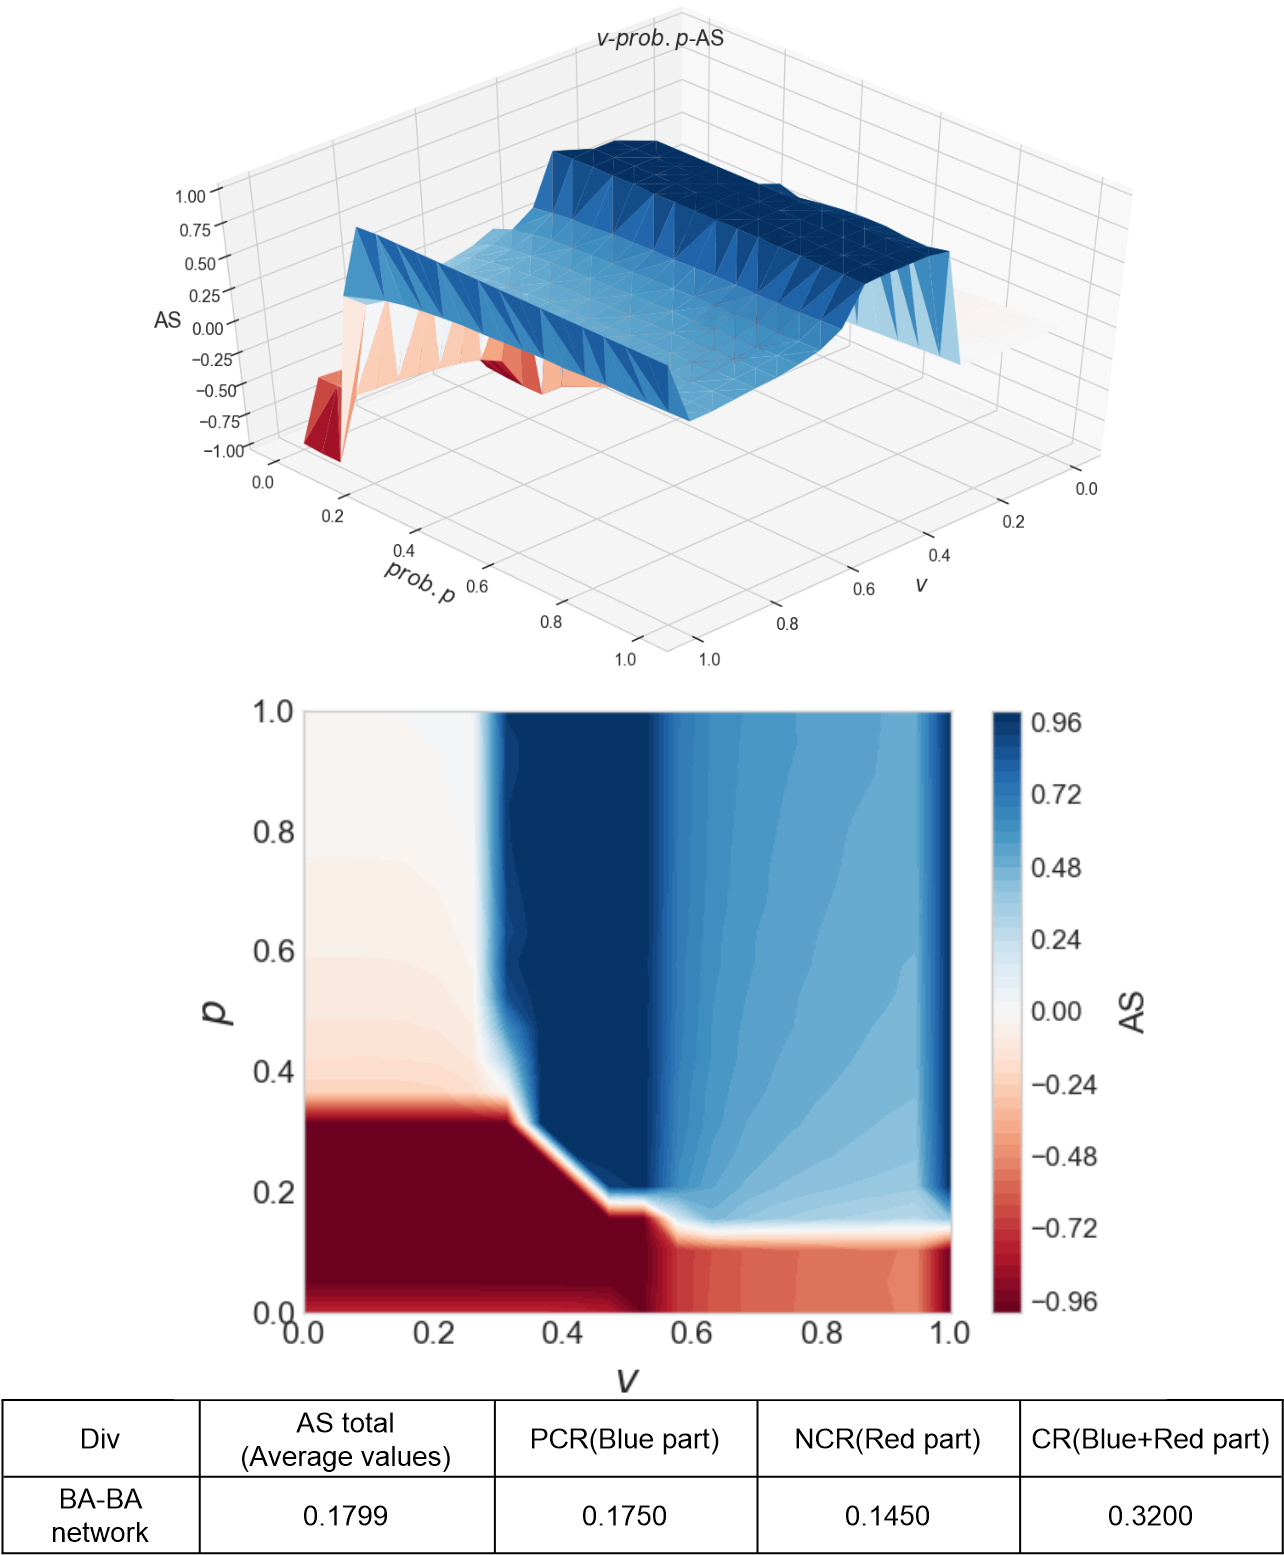
\includegraphics[width=\hsize]{chap2_AS_total(BA3_BA3).png}
	\caption{The example of simulation : BA-BA network}
	\label{chap2_AS_total(BA3_BA3)}
\end{figure}

Fig.~\ref{chap2_AS_total(BA3_BA3)} shows the states of interconnected network according to all $p$s and all $v$s. The $X$-axis is the $p$ and the $Y$-axis is the $v$, and the $Z$-axis represents \textit{AS}. The closer the color is to blue, the more it has positive consensus. And the closer the color is to red, the more it has negative consensus. A light colored and white areas have coexistence with positive states and negative states. Here, we can measure the consensus by using indexes, \textit{`AS total'}, \textit{`PCR'}, \textit{`NCR'}, and \textit{`CR'}. The average value of this figure means \textit{`AS total'}. The blue part area means \textit{`PCR'}, the red part area means \textit{`NCR'}, and the summation of those means \textit{`CR'}. 



    
